
\chapter{Mise en oeuvre de \PpFf}
\label{implementation.chap}


\gt{Avant d'avoir une subsection, tu dois avoir une section. Donc, v\'erifie la structure de ce chapitre!}

\ic{J'ai ajout\'e une petite introduction du chapitre.}

\begin{figure}[ht]
\centering
     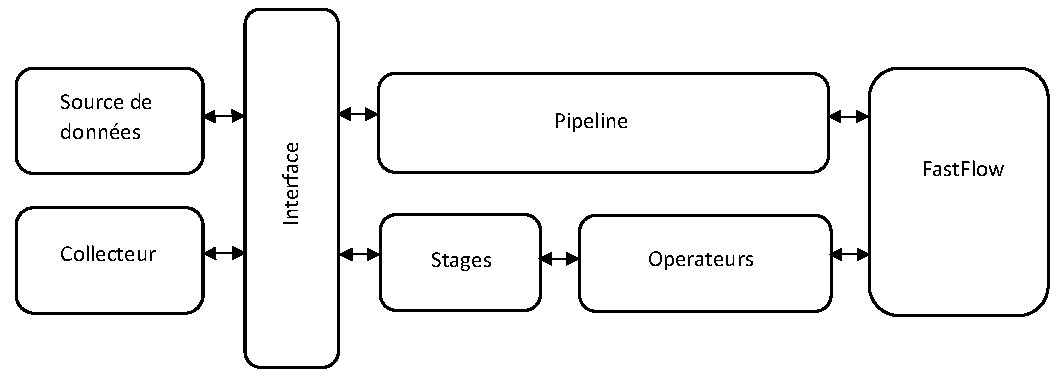
\includegraphics[width=1.0\textwidth]{Figures/AllComponentsAPI.jpg}
      \caption{Les composants de \TT{PpFf}.}
       \label{AllComponentsAPI.fig}
\end{figure}


Ce chapitre donne une description plus d\'etaill\'ee de la fa\c{c}on dont \TT{PpFf} est impl\'ement\'e. Une vue d'ensemble de ses composants est pr\'esent\'ee à la figure~\ref{AllComponentsAPI.fig}. De fa\c{c}on g\'en\'erale, la mise en \oe{}uvre est bas\'ee sur la biblioth\`eque \TT{FastFlow}, h\'eritant et \'etendant plusieurs de ses classes. La premi\`ere section montre les couches de l'API et les liaisons entre elles.  La deuxi\`eme section d\'ecrit comment le pipeline du flux est mis en œuvre. La section suivante examine comment la parall\'elisation du flux est r\'ealis\'ee. Les stages sont d\'ecrits dans la quatri\`eme section. Le chapitre se termine par la description d'un exemple complet d\'ecrivant comment un programme PpFf est compil\'e et ex\'ecut\'e.


\section{Mise en \oe{}uvre multi-couches de \PpFf{} via FastFlow}

\GT{De quelle fa\c{c}on as-tu fait le diagramme?  Est-ce que ce serait
possible, dans la partie du haut surtout, de changer l'ordre de
pr\'esentation des classes? Cela aurait plus de sens de mettre la
classe Pipe en haut, puisque c'est la classe principale.  Et on ne
comprend pas trop pourquoi il y a Pipe, PipeManager et Pipeline?
D'autant plus que dans la figure 3.1, il y aussi Stage, qui n'apparait
pas dans la figure 3.2. Et en relisant, je constate que dans la figure
2.1, il y a Pipeline et Operateurs, mais il n'y a pas Stage.  Tout
cela semble un peu m\'elangeant~:(}

\IC{J'ai redessin\'e le diagramme et j'ai ajout\'e une autre pour les stages dans la section Stage~\ref{StagesClassDiagramme.fig}.}


\begin{figure}[ht]
\centering
     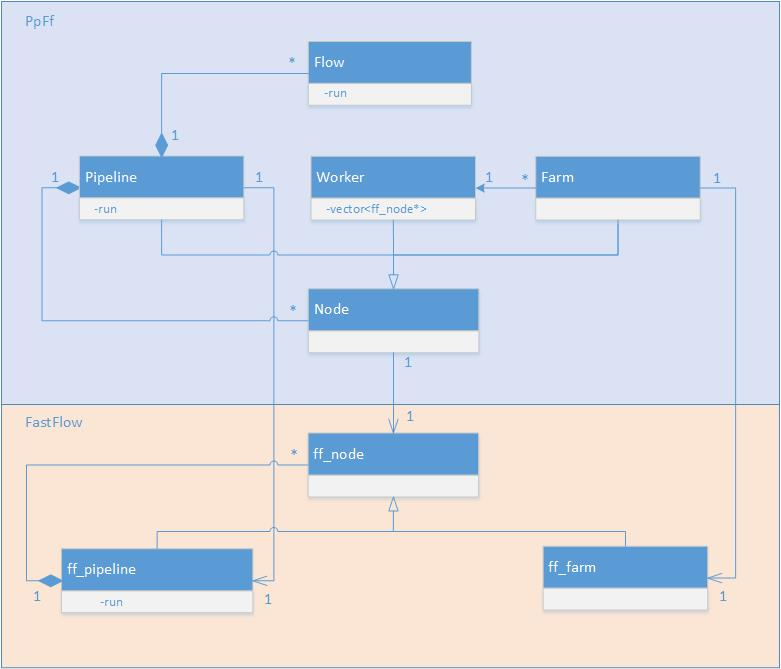
\includegraphics[width=1.0\textwidth]{Figures/CorrespondencePpFfToFastFlow.jpg}
      \caption{La correspondance entre les \'el\'ements de \TT{PpFf} et ceux de  \TT{FastFlow}.}
       \label{CorrespondencePpFfToFastFlow.fig}
\end{figure}


%\begin{figure}[ht]
%\centering
%     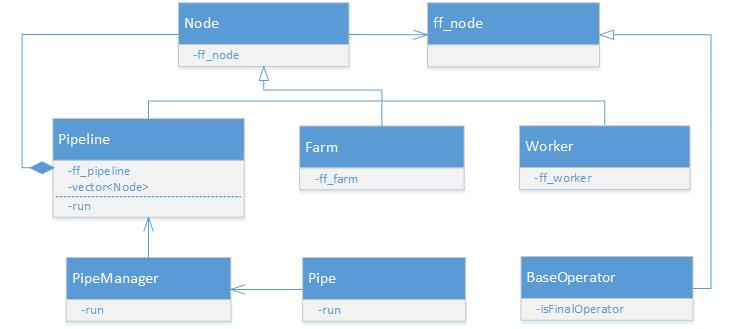
\includegraphics[width=1.0\textwidth]{Figures/MapToFastFlow.jpg}
%      \caption{La correspondance entre les \'el\'ements de \TT{PpFf} et ceux de  \TT{FastFlow}.}
%       \label{MapToFastFlow.fig}
%\end{figure}


PpFf est impl\'ement\'e au--dessus de la biblioth\`eque \TT{FastFlow}, de sorte que nous utilisons les constructions \TT{ff\_node}, \TT{ff\_pipeline} et \TT{ff\_farm} de \TT{FastFlow}. La figure~\ref{CorrespondencePpFfToFastFlow.fig} montre la correspondance entre les \'el\'ements de \TT{PpFf} et ceux de \TT{FastFlow}. Chaque classe susmentionn\'ee de \TT{FastFlow} a une association dans \TT{PpFf}. Par exemple l'impl\'ementation de la classe \TT{Node} de \TT{PpFf} est r\'ealis\'ee par l'entremise de la classe \TT{ff\_node} de \TT{FastFlow}. Ce m\'ecanisme a permis d'ajouter plus de fonctionnalit\'e \`a l'API tout en utilisant les performances offertes par \TT{FastFlow}.


\GT{Ci-haut: le texte parle de correspodance, sauf qu'il n'y a pas du
tout de lien (graphique) entre les deux niveaux~:( Peut-\^etre
faudrait-il montrer des liens graphiques? Par exemple, pour Farm, au
lieu d'avoir un attribut \TT{ff\_farm}, faudrait-il avoir un lien vers
la classe \TT{ff\_farm}? C'est certain que le graphique serait plus
compliqu\'e, donc peut-\^etre le faire par morceau? Ou dans l'autre
sens (landscape)?}

\IC{J'ai repr\'esent\'e la correspondance par une ligne pointill\'ee.}


\section{Pipeline}

Tel que mentionn\'e au chapitre pr\'ec\'edent, un pipeline est compos\'e d'une cha\^ine de traitement appel\'e \TT{Pipeline}. Un \TT{Pipeline} est repr\'esent\'e essentiellement par une s\'erie d'op\'erateurs d\'efinis par l'utilisateur qui sont appliqu\'es aux \'el\'ements d'un flux. Comme on peut le voir dans la figure~\ref{CorrespondencePpFfToFastFlow.fig}, un \TT{Pipeline} implemente les fonctionnalit\'ees de la class \TT{ff\_pipeline} de \TT{FastFlow}. 

Tel que d\'ecrit au chapitre pr\'ec\`edent, les op\'erateurs qui composent un \TT{Pipeline} sont de deux types : les op\'erateurs sans \'etat et les op\'erateurs avec \'etat. Un \TT{Pipeline} contient un ou plusieurs op\'erateurs sans \'etat et un seul op\'erateur avec \'etat. Lorsque ce dernier est ajout\'e dans le \TT{pipeline}, la m\'ethode \TT{run()} est appel\'ee. \`A ce stade, un objet de type \TT{ff\_pipeline} correspondant au \TT{Pipe} est cr\'e\'e. Ensuite, chaque op\'erateur d\'efini par l'utilisateur est visit\'e et, en fonction de la configuration \'etablie, des objets de type \TT{ff\_node} ou \TT{ff\_farm} sont ajout\'es dans l'objet \TT{ff\_pipeline}. Chaque nœud ainsi ajout\'e dans \TT{ff\_pipeline} sera ex\'ecut\'e dans un fil d'ex\'ecution ind\'ependant, une caract\'eristique de la mise en \oe{}uvre de \TT{FastFlow}.
La cr\'eation de \TT{Pipeline} est r\'ealis\'ee \`a l'aide de \TT{PipeManager}.


\section{Parall\'elisation}

La cr\'eation de code parall\`ele est g\'en\'eralement consid\'er\'ee du domaine d'experts. La complexit\'e du code parall\`ele diminue la productivit\'e, ce qui peut augmenter les co\^uts de d\'eveloppement. \TT{PpFf} permet aux programmeurs de composer du code s\'equentiel et de l'ex\'ecuter en parall\`ele. Par l'interm\'ediaire d'une interface unique, l'API offre deux mod\`eles de parall\'elisme : le parall\'elisme de t\^aches et le parall\'elisme de donn\'ees.

\gt{Si tu parles de <<parall\'elisme de flux>>, alors tu devrais
parler de <<parall\'elisme de t\^aches>>, ou <<parall\'elisme de
donn\'ees>>. Un Task-Farm est un m\'ecanisme sp\'ecifique pour mettre
en oeuvre une de ces deux derni\`eres formes de parall\'elisme.}

\ic{J'ai d\'ecrit le parall\'elisme de t\^aches et parall\'elisme de donn\'ees plut\^ot que le parall\'elisme de flux.}


\subsection{Parall\'elisme de t\^aches}

Le parall\'elisme de t\^aches consiste \`a ex\'ecuter plusieurs \'etapes d'un traitement s\'equentiel en parall\`ele en leur faisant traiter des données diff\`erentes. Les donn\'ees se succ\`edent ainsi les unes aux autres dans les diff\'erentes \'etapes --- appel\'ees  aussi des \emph{stages}~\ref{stages.sect}. \`A noter que ce type de parall\'elisme est appliqu\'e par d\'efaut dans notre API. Le traitement effectu\'e dans un \emph{stage} \`a un instant donn\'e peut d\'ependre des traitements effectu\'es par ce m\^eme \emph{stage} pour les donn\'ees pr\'ec\'edentes --- un \'etat interne peut donc \^etre conserv\'e. Ce fonctionnement permet de parall\'eliser des traitements avec de fortes d\'ependances entre les donn\'ees sans avoir recours \`a de nombreuses synchronisations. 

Un flux avec $n$ \emph{stages} peut \^etre formellement exprim\'e sous la forme d'une composition s\'equentielle d'op\'erateurs sur les \'el\'ements d'entr\'ee comme suit~: 

\[
	O(x) = O_n( \ldots (O_k( \ldots O_1(x)) \ldots ) \ldots ));
\]


\begin{figure}[ht]
\centering
     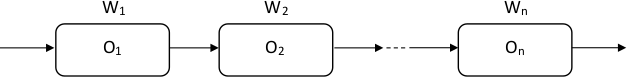
\includegraphics[width=1.0\textwidth]{Figures/ParallelismeDuFlux.jpg}
      \caption[Une repr\'esentation graphique du parall\'elisme de t\^aches.]{Une repr\'esentation graphique du parall\'elisme de t\^aches pour une d\'ecomposition en $n$ \emph{stages} $S_1, S_2, \ldots, S_n$. Les op\'erations $O_1, O_2, \ldots, O_n$ sont ex\'ecut\'ees de fa\c{c}on concurrente dans des diff\'erents fils d'ex\'ecution $W_1, W_2, \ldots, W_n$ ($W$ pour \emph{$W$orker}).}
       \label{ParallelismeDuFlux.fig}
\end{figure}


Dans ce cas, le parall\'elisme est repr\'esent\'e par un graphe lin\'eaire de $n$ travailleurs. Chaque travailleur correspond \`a une op\'eration sp\'ecifique. La figure~\ref{ParallelismeDuFlux.fig} montre la repr\'esentation graphique du parall\'elisme de t\^aches. Cette solution n'acc\'el\`ere pas le calcul d'un seul \'el\'ement. Par contre, elle am\'eliore le d\'ebit de sortie.

\subsection{Parall\'elisme de donn\'ees}

Le parall\'elisme de donn\'ees impl\'ement\'e dans \TT{PpFf}  consiste \`a r\'epliquer un op\'erateur parmi un ensemble de travailleurs identiques. Autrement dit, il vise \`a effectuer un traitement identique sur un ensemble de donn\'ees ind\'ependantes les unes des autres. 
%
Dans notre impl\'ementation de \PpFf, le parall\'elisme de donn\'ees est mis en oeuvre avec les \emph{Task Farm} de FastFlow.


D\'ecrit \`a la section~\ref{farm.sect}, un \emph{Task Farm} est compos\'ee de trois entit\'es : un \TT{Emitter}, plusieurs instances de travailleurs (\emph{workers}) et un \TT{Collector}. Par d\'efaut, dans \PpFf{} les \'el\'ements sont r\'epartis par un \TT{Emitter} aux divers travailleurs selon une politique \emph{round robin}. Les travailleurs re\c{c}oivent les \'el\'ements d'entr\'ee et appliquent sur chacun l'op\'erateur d\'efini au pr\'ealable par l'utilisateur. Les r\'esultats sont ensuite envoy\'es vers le \TT{Collector} charg\'e de les collecter --- i.e., de les combiner --- puis de les transmettre au flux de sortie.

Dans \TT{PpFf}, les \'el\'ements du flux sont trait\'es dans l'ordre d'arriv\'ee selon le principe \emph{FIFO}. La collection de plusieurs r\'esultats \`a l'aide de cette approche r\'esulte dans un flux sans ordre sur ses \'el\'ements. En effet, le \TT{Collector} transmet les \'el\'ements au flux de sortie dans l'ordre d'arriv\'ee. \'Etant donn\'e que plusieurs flux ind\'ependants sont impliqu\'es, cet ordre ne peut pas \^etre pr\'ed\'etermin\'e. Si le respect d'un  ordre sp\'ecifique est requis, l'utilisateur de l'API peut ajouter un op\'erateur qui produit cet ordre. Par exemple, la m\'ethode \TT{sort} de l'API, d\'efinie dans le tableau~\ref{methodes_api.tab}, effectue le tri des \'el\'ements du flux selon l'ordre sp\'ecifi\'e par la fonction \TT{compare} envoy\'e en param\`etre.

\goodbreak
%
\begin{samepage}
L'impl\'ementation parall\`ele de ce mod\`ele peut \^etre formellement
exprim\'ee sous la forme d'un ensemble de travailleurs $W_1, W_2,\ldots, W_n$ qui
appliquent l'op\'erateur $O$ sur les \'el\'ements $X$ apparaissant dans
le flux d'entr\'ee~:
%
\[
	W_1, W_2,\ldots, W_n
\]
%
\[
	O : X_i \rightarrow Y_i
\]
\end{samepage}

\begin{figure}[ht]
\centering
     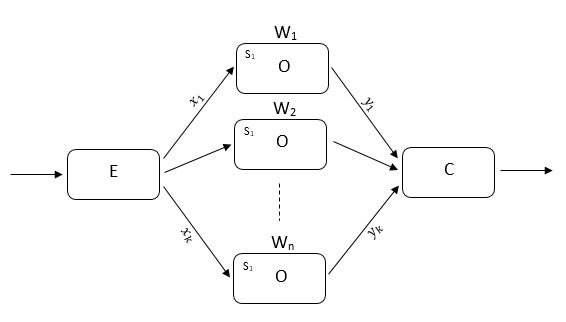
\includegraphics[width=1.0\textwidth]{Figures/DataParallelisme.jpg}
      \caption[Une repr\'esentation graphique du parall\'elisme de donn\'ees.]{Une repr\'esentation graphique du parall\'elisme de donn\'ees. La m\^eme op\'eration $O$ est ex\'ecut\'ee par les travailleurs $W_1, W_2,\ldots, W_n$ ($W$ pour \emph{$W$orker}). Le traitement associ\'e est repr\'esent\'e logiquement par le stage $S_1$. Les \'el\'ements de donn\'ees sont r\'epartis entre les travailleurs par l'\'emetteur ($E$\emph{mitter}). Les divers r\'esultats sont ensuite combin\'es par le collecteur $C$.}
       \label{DataParallelisme.fig}
\end{figure}


Le r\'esultat $Y_i$ est g\'en\'er\'e en appliquant l'op\'erateur $O$ sur l'\'el\'ement $X_i$. La figure~\ref{DataParallelisme.fig} montre une repr\'esentation graphique du parall\'elisme de donn\'ees. Le m\^eme op\'erateur est ex\'ecut\'e par les travailleurs $W_1, W_2,\ldots, W_n$. 

Il est possible de sp\'ecifier, en param\`etre, le nombre de travailleurs \`a utiliser pour l'ex\'ecution parall\`ele. Si ce param\`etre n'est pas sp\'ecifi\'e, un seul travailleur est activ\'e. Cette solution de permettre d'augmenter le nombre de travailleurs fait en sorte qu'on peut augmenter le d\'ebit du traitement des donn\'ees si appropri\'e, c'est-\`a-dire, augmenter le nombre de donn\'ees qui peuvent \^etre trait\'ees en un temps donn\'e.




\section{Stages}
\label{stages.sect}

\GT{Bon, je vais devoir faire une autre lecture de cette partie plus tard, car je ne suis pas certain encore de bien comprendre \frownie}

\IC{Dans le cas du parall\'elisme de donn\'ees, on applique un Farm. Un Farm est compos\'e d'un Emmiter, les workers et un Collector. Lorsque le parall\'elisme est appliqu\'e sur les op\'erateurs finals (op\'erateurs avec \'etat) j'ai enlev\'e le Collector. Par exemple si on applique une op\'erateur de r\'eduction sur 4 threads, chaque thread va contenir le r\'esultat partiel de la r\'eduction. Afin de combiner les 4 r\'esultats, j’avais besoin d'un m\'ecanisme qui envoyait ces valeurs au Collector \`a la fin du flux. Dans FastFlow la fin du flux est signal\'ee par la valeur EOS. Lorsque cette valeur est propag\'ee dans le flux, le flux s'arr\^ete. J'ai essay\'e la variante suivante : v\'erifier si cette valeur est envoy\'ee dans le flux et dans le cas affirmatif envoyer les 4 r\'esultats au Collector, mais cette solution n'a pas fonctionn\'e. Si je me rappelle bien, le Collector \'etait \`a vide.} 

\IC{La solution que j'ai trouv\'ee \'etait d'enlever le Collector et de combiner les 4 r\'esultats dans l'impl\'ementation de la class Stage.}

\begin{figure}[ht]
\centering
     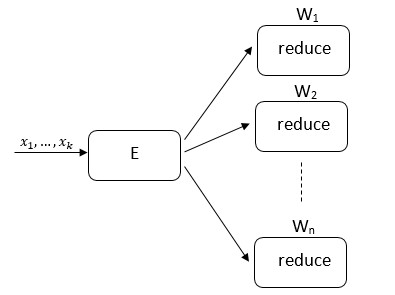
\includegraphics[width=0.8\textwidth]{Figures/StageDataParallel.jpg}
      \caption[Un exemple d'application de l'op\'erateur \TT{reduce} sur diff\'erents sous-flux de donn\'ees.]{Un exemple d'application de l'op\'erateur \TT{reduce} sur diff\'erents sous-flux de donn\'ees. L'\TT{Emitter} E distribue  les \'el\'ements des sous-flux de donn\'ees aux diff\'erents fils d'ex\'ecution $W_1, W_2, \ldots, W_n$.}
       \label{StageDataParallel.fig}
\end{figure}

Le traitement en parall\`ele d'un flux de donn\'ees contribue \`a augmenter les performances du pipeline en utilisant les diff\'erents cœurs de la machine. Cependant, il existe une limitation lorsque le parall\'elisme de donn\'ees est appliqu\'e sur certains op\'erateurs. Dans un flux, seuls les op\'erateurs sans \'etat peuvent \^etre parall\'elis\'es en toute s\'ecurit\'e. Par contre, quand il est n\'ecessaire de parall\'eliser un op\'erateur avec \'etat, les choses deviennent un peu plus compliqu\'ees parce que le r\'esultat du calcul est obtenu en traitant un ensemble d'\'el\'ements d'entrée appartenant \`a un ou plusieurs flux de donn\'ees. Par exemple, la figure~\ref{StageDataParallel.fig} montre un exemple o\`u l'op\'erateur \TT{reduce} est appliqu\'e en parall\`ele. Le r\'esultat global est obtenu en combinant les r\'esultats du traitement de chacun des sous-flux trait\'es dans un fil d'ex\'ecution ind\'ependant. Afin d'optimiser le traitement, nous avons introduit les \emph{stages}.

%Comme la plupart des traitements consistent en une combinaison d'op\'erateurs avec ou sans \'etat, un traitement parall\`ele ne peut pas \^etre effectu\'e. Une solution consiste alors \`a parall\'eliser les op\'erateurs sans \'etat et \`a utiliser un op\'erateur \TT{Collector} pour fusionner les flux parall\`eles avant d'appliquer un op\'erateur avec \'etat. Cette solution implique l'utilisation d'un autre cœur de la machine. De plus, le traitement pour les op\'erateurs avec \'etat est effectu\'e de fa\c{c}on s\'equentielle. Afin d'optimiser le traitement, nous avons introduit les \emph{stages}.

\begin{figure}[ht]
\centering
     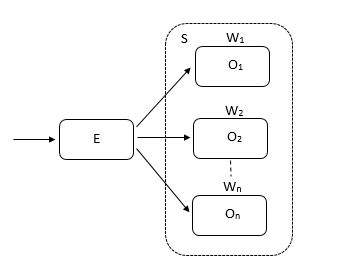
\includegraphics[width=0.8\textwidth]{Figures/Stages.jpg}
      \caption[Le groupement logique de $n$ op\'erateurs $O_1, O_2, \ldots, O_n$ dans un \TT{stage} S.]{Le groupement logique de $n$ op\'erateurs $O_1, O_2, \ldots, O_n$ dans un \TT{stage} S.  L'\TT{Emitter} E distribue les \'el\'ements du flux aux diff\'erents fils d'ex\'ecution $W_1, W_2, \ldots, W_n$.}
       \label{Stages.fig}
\end{figure}

\begin{figure}[ht]
\centering
     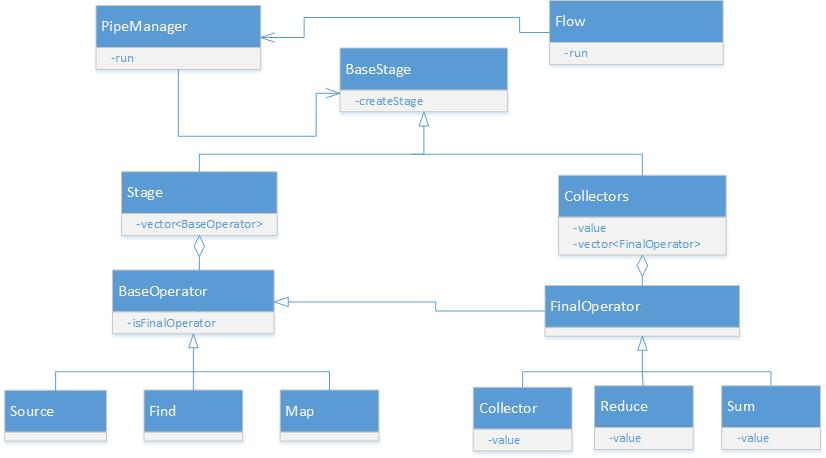
\includegraphics[width=1.0\textwidth]{Figures/StagesClassDiagramme.jpg}
      \caption{La diagramme de classe pour Stage.}
       \label{StagesClassDiagramme.fig}
\end{figure}


Un \emph{stage} repr\'esente le groupement logique d'un ou plusieurs op\'erateurs d'une \'etape dans la cha\^ine de traitement d'un pipeline. La figure~\ref{Stages.fig} montre plusieurs op\'erateurs finaux group\'es logiquement dans un stage.  \`A noter que ce module n'est pas visible \`a l'utilisateur. Dans \TT{PpFf}, nous distinguons deux types de \emph{stages} : les \emph{stages} interm\'ediaires et les \emph{stages} finaux. Comme leur nom le sugg\`ere, les \emph{stages} interm\'ediaires groupent seulement les op\'erateurs sans \'etat et les \emph{stages} finaux groupent les op\'erateurs finaux. La figure~\ref{StagesClassDiagramme.fig} montre la diagramme de classe pour \emph{stages}. Dans le cas du traitement parall\`ele, les \emph{stages} finaux ont pour r\^ole de r\'eduire l'\'etat d'op\'erateurs finaux de chaque fil d'ex\'ecution selon l'op\'eration donn\'ee. La valeur issue du flux repr\'esente le r\'esultat du traitement du flux de donn\'ees.



\section{Impl\'ementation de \TT{PpFf} avec FastFlow: Un exemple}

\begin{lstlisting}[
label={listingExampleImplementationPpFf},
language=c++,
caption={[Le code source d'une petite application.]Le code source d'une petite application utilis\'ee pour d\'ecrire l'impl\'ementation de PpFf.},
frame=single,
float]
auto convert_to_lowercase = [](std::string* data) {
  std::string* result = new std::string;
  for (char c: *data) {
    if ('a' <= c && c <= 'z') {
   	  result->push_back(c);
   	} else if ('A' <= c && c <= 'Z') {
	  result->push_back(c-('Z'-'z'));
   	}
  }
  return result;	
};

auto find_not_empty = [](std::string* s) {
  return s->size() > 0;
};
	
std::vector<std::string> result = 
  Flow
  ::source(path)
  .find<std::string>(find_not_empty)
  .parallel(2)
  .map<std::string, std::string>(convert_to_lowercase)
  .collect<std::string, std::vector>();
\end{lstlisting}


\GT{Suggestion pour le code source du Listing 3.1~: Oui, donner le
code des lambda-expressions, mais introduire explicitement des
lambda-expressions avec un nom, ce qui aidera \`a comprendre ce que
cela fait, par ex., d\'eclarer une variable lambda-expression {\bf
avant} de d\'efinir result~: <<auto mettre\_en\_minuscules =
[](std::string* s)...>>, puis map<std::string,
std::string>(mettre\_en\_minuscules). Idem pour l'autre
lambda-expression utilis\'ee dans le find.}

\IC{J'ai ajout\'e des lambda--expressions avec un nom.}

Cette section d\'ecrit le mod\`ele d'ex\'ecution de \ppff\ \`a l'aide du code source d'une petite application. Illustr\'ee dans le listing~\ref{listingExampleImplementationPpFf}, l'application est compos\'ee des op\'erations suivantes :
\begin{itemize}
	\item L'opération \TT{linesFromFile} g\'en\`ere un flux séquentiel de lignes à partir d'un fichier --- le fichier est identifi\'e par le paramètre \TT{path} fourni en argument;

	\item L'op\'eration \TT{find} s\'electionne dans le flux d'entr\'ee les mots qui ne sont pas vides;

	\item L'op\'eration \TT{parallel} indique que les op\'erations subs\'equentes doivent \^etre ex\'ecut\'ees en parall\`ele, ici, avec deux \emph{threads};
	
	\item L'op\'eration \TT{map} transforme les lettres majuscules du mot en lettres minuscules;
	
	\item Finalement, l'op\'eration \TT{collect} combine tous les \'el\'ements obtenus dans un conteneur de type \TT{vector}.
\end{itemize}

\GT{Je crois qu'il serait pr\'ef\'erable, <<par souci de compl\'etude>> et pour assurer que le lecteur comprenne bien ce que fait le programme, de fournir aussi ces fonctions, quitte \`a les d\'efinir simplement sous forme d'expression-lambda.}

\IC{J'ai impl\'ement\'e les fonctions sous forme d'expression-lambda.}


\begin{figure}[ht]
\centering
     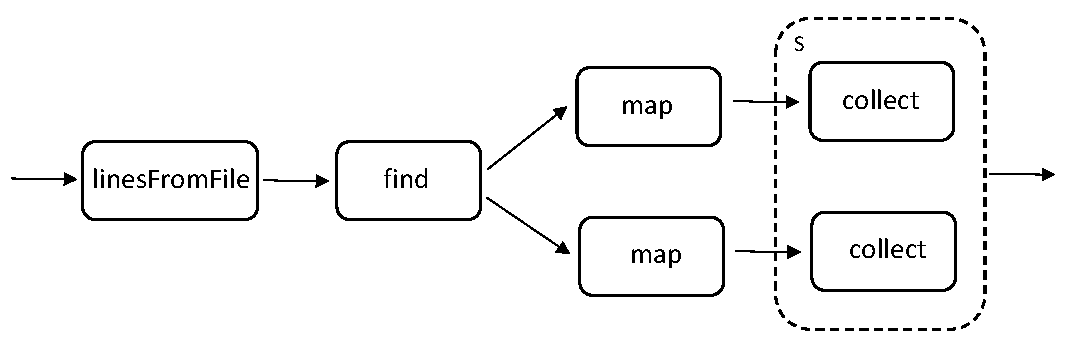
\includegraphics[width=0.8\textwidth]{Figures/ExempleRuntimeExecution.jpg}
      \caption[Repr\'esentation graphique d'un \TT{pipeline} compos\'e de quatre op\'erateurs.]{Repr\'esentation graphique d'un \TT{pipeline} compos\'e de quatre op\'erateurs ex\'ecut\'es en parall\`ele. Le mod\`ele de parall\'elisme de t\^aches est appliqu\'e sur les deux premiers op\'erateurs et le mod\`ele de parall\'elisme de donn\'ees est appliqu\'e sur les derniers op\'erateurs.}
       \label{ExempleRuntimeExecution.fig}
\end{figure}

\GT{Le probl\`eme avec la figure 3.8 est qu'on ne voit pas
explicitement/clairement les objets fastflow qui sont g\'en\'er\'es:
Est-ce que Lff est un ff\_node, un ff\_pipeline, etc. Idem pour les
autres.  Il faudrait voir plus clairement et explicitement les objets
FastFlow (ff\_node, ff\_pipeline, ff\_farm, etc.) et leurs liens.}


La classe \TT{Pipeline} de l'API repr\'esente l'entit\'e principale de l'application. \`A l'ex\'ecution, le \TT{Pipeline} correspond \`a la classe \TT{ff\_pipeline} de \TT{FastFlow}. Un \TT{Pipeline} est compos\'e de plusieurs nœuds de type \TT{ff\_node} ou \TT{ff\_farm}. La figure~\ref{ExempleRuntimeExecution.fig} montre la repr\'esentation graphique d'un \TT{Pipeline} compos\'e des op\'erateurs d\'ecrits dans le listing~\ref{listingExampleImplementationPpFf}.
 
Dans un \TT{Pipeline}, le premier op\'erateur est toujours un op\'erateur d'entr\'ee, lequel est impl\'ement\'e sous forme d'un \TT{ff\_node}. Dans notre exemple, \TT{linesFromFile} renvoie un flux s\'equentiel de lignes \`a partir d'un fichier. De plus, l'op\'erateur d'entr\'ee a aussi la t\^ache d'envoyer un signal \TT{EOS} lorsque la g\'en\'eration d'entr\'ee est termin\'ee~: \TT{EOS} indique aux nœuds \TT{ff\_node}s de \TT{FastFlow} de terminer leur ex\'ecution apr\`es la r\'eception de celui-ci.

La classe repr\'esentant chaque nœud dans un \TT{Pipeline} contient les informations concernant son r\^ole dans la chaine du traitement. Par exemple, l'op\'erateur \TT{find} du listing~\ref{listingExampleImplementationPpFf} a pour r\^ole de s\'electionner dans le flux seulement les mots qui ne sont pas vides. Ce r\^ole est d\'efini par l'utilisateur \`a la cr\'eation du \TT{Pipeline}, en fournissant une fonction ou lambda-expression \`a \TT{find}.


Les divers op\'erateurs d'un \TT{Pipeline} sont toujours ex\'ecut\'es en parall\`ele.  Rappelons que, dans \TT{FastFlow}, chaque \TT{ff\_node} est associ\'e \`a un \emph{thread} ind\'ependant. Le mod\`ele de parall\'elisme de t\^aches --- plus sp\'ecifiquement, de flux --- est donc appliqu\'e par d\'efaut. 

En outre, lorsqu'un appel \`a la m\'ethode \TT{parallel} est ajout\'e dans la chaine du traitement d'un \TT{Pipeline}, les op\'erateurs subs\'equents sont ex\'ecut\'es en parall\`ele, et ce en utilisant du parall\'elisme de donn\'ees. Dans l'exemple du listing~\ref{listingExampleImplementationPpFf}, les deux premiers op\'erateurs sont ex\'ecut\'es en parall\`ele, avec du parall\'elisme de t\^aches, alors que du parall\'elisme de t\^aches et du parall\'elisme de donn\'ees sont aussi exploit\'es pour les op\'erateurs suivants (apr\`es \TT{parallel}). 

\begin{figure}[ht]
\centering
     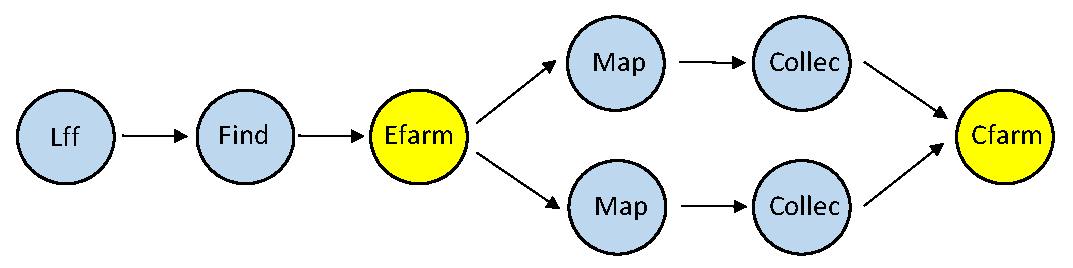
\includegraphics[width=0.8\textwidth]{Figures/ExempleRuntimeExecutionFF.jpg}
      \caption[Repr\'esentation graphique du listing~\ref{listingExampleImplementationPpFf} en \TT{FastFlow}.]{Repr\'esentation graphique du listing~\ref{listingExampleImplementationPpFf} en \TT{FastFlow}. Les cercles bleus repr\'esentent les op\'erateurs d\'efinis par l'utilisateur : \TT{lineFromFile} (Lff), \TT{find} (Find), les deux \TT{map} (Map) et les deux \TT{collector} (Collec). Les cercles en jaunes repr\'esentent l'\TT{Emitor} et le \TT{Collector} de \TT{ff\_farm}.}
       \label{ExempleRuntimeExecutionFF.fig}
\end{figure}

Dans l'impl\'ementation de \TT{PpFf}, le parall\'elisme de donn\'ees est mis en œuvre avec la classe \TT{ff\_farm} de \TT{FastFlow}. La cr\'eation du flux de traitement en utilisant le mod\`ele de parall\'elisme de donn\'ees est simple. Lorsque la m\'ethode \TT{parallel()} est invoqu\'ee, une instance de la classe \TT{ff\_farm} est ajout\'ee dans le \TT{Pipeline}. Pour chaque \emph{worker} de \TT{ff\_farm}, un nouveau \TT{ff\_pipeline} est cr\'e\'e. Les op\'erateurs ajout\'es dans la chaine du traitement  sont ajout\'es comme nœuds dans les nouveaux \TT{ff\_pipeline} cr\'e\'es. Par exemple, les op\'erateurs \TT{map} et \TT{collect} du listing~\ref{listingExampleImplementationPpFf} sont ajout\'es dans le \TT{pipeline} de chaque \TT{worker} de \TT{ff\_farm}. La figure~\ref{ExempleRuntimeExecutionFF.fig} montre la repr\'esentation graphique de \TT{FastFlow}. Chaque cercle est une classe de type \TT{ff\_node}. Les cercles en bleu repr\'esentent les op\'erateurs d\'efinis par l'utilisateur : \TT{lineFromFile} (Lff), \TT{find} (Find), les deux \TT{map} (Map) et les deux \TT{collector} (Collec). Les cercles en jaunes repr\'esentent l'\TT{Emitor} et le \TT{Collector} de \TT{ff\_farm}. 


\GT{Ce serait int\'eressant --- est-ce possible ou trop compliqu\'e? --- de montrer une repr\'esentation graphique du pipeline FastFlow ainsi g\'en\'er\'e! Dans ce cas, on verrait alors mieux les \'el\'ements FastFlow qui correspondent aux op\'erateurs PpFf.}

\IC{J’ai ajout\'e un diagramme pour montrer le flux dans FastFlow.}

L'ex\'ecution parall\`ele d'un flux est r\'ealis\'ee par l'ex\'ecution de la m\'ethode \TT{run\_and\_wait\_end()} de la classe \TT{ff\_pipeline} de \TT{FastFlow}. Chaque \TT{ff\_node} de \TT{ff\_pipeline} est une instance de la classe C++ \TT{ff\_node} qui, dans sa m\'ethode \TT{svc()},  ex\'ecute une boucle de traitement qui va comme suit:
\begin{itemize}
	\item elle obtient du canal d'entr\'ee, via un pointeur, un \'el\'ement \`a traiter;
	\item elle ex\'ecute le code sur l'\'el\'ement;
	\item elle \'emet dans le canal de sortie,  via un pointeur,  l'\'el\'ement produit;
\end{itemize}

Les nœuds d'un pipeline sont ex\'ecut\'es jusqu'\`a ce qu'ils re\c coivent le signal \TT{EOS} (\emph{End-Of-Stream}). \`A ce moment, tous les nœuds sont d\'etruits. Dans le cas de noeuds multiples associ\'es au de parall\'elisme de donn\'ees, le r\'esultat global de l'op\'erateur est obtenu en combinant les r\'esultats de chacun des sous-flux, produits par les divers fils d'ex\'ecution. Par exemple, chaque op\'erateur \TT{collect} repr\'esent\'e dans la figure~\ref{ExempleRuntimeExecution.fig} collecte le r\'esultat du traitement de chacun des sous-flux trait\'es dans un fil d'ex\'ecution ind\'ependant. Le r\'esultat global est obtenu via la classe \TT{Stage} qui combine ces r\'esultats interm\'ediaires.
